\label{changelog20200901_nop3}

\chapter{Processors}

Special-case information, and tips and tricks for the processors supported by \dasm are described here.

\section{The 6502 Processor}

\subsection{Support for Illegal Opcodes}

The effects of the ``unused'' opcodes on the 6502 are by now relatively well documented. These are variously described as illegal, undocumented, invalid, and unspecified. Modern programs use some of these, as they provide additional capabilities (particularly speed improvements) over the use of the standard opcodes. \dasm explicitly supports some of the commonly used `stable' illegal opcodes, and those are listed below. In this table, LL references the low byte of a 16-bit value, and HH the high byte.)

\url{http://www.oxyron.de/html/opcodes02.html} provides a good table of the opcodes and their mnemonics.  Some of the illegal opcodes shown in Figure \ref{fig:IllegalOp}  are not supported by \dasm.

%\includegraphics[width=1\textwidth]{images/illegal}
\begin{landscape}
\begin{figure}[h]
\centering
\includegraphics[width=1\linewidth]{../DASM/images/illegal}
\caption{Illegal Opcodes. \textcopyright 2002-2012 Graham\\Retrieved from \url{http://www.oxyron.de/html/opcodes02.html} on 2020.09.01\\
}
\label{fig:IllegalOp}
\end{figure}

\end{landscape}

\subsubsection{Example}
\begin{code}
  PROCESSOR 6502
  org $1000
  nop 0       ; insert byte sequence \$04 \$00
  lax $1000   ; loads bot A and X registers with 4
\end{code}



\chapter{The Machines}

\dasm supports specific machinesand processors through the provision of additional source-code files that can assist with programming each platform. These files are located in the \mono{machines} subdirectory. Support is provided for...

\begin{itemize}
\item \nameref{machine:atari2600}
\item Atari 7800
\item Channel F
\item 68hc11
\item 68hc908
\end{itemize}


\section{Atari 2600}
\label{machine:atari2600}

The Atari 2600 is a game console from 1978 that uses a 6507 processor. This processor is similar to the 6502 processor (supported by \dasm). The difference in the processors is the number of hardware address lines on the chips; these being 16 on the 6502, and 12 on the 6507. Thus, the 6502 can directly address 64K of memory and the 6507 only 4K of memory.  From the point of view of \dasm, the machines are identical, as the 6502 and 6507 share a common instruction set.

For programming the Atari 2600, use \mono{PROCESSOR 6502} at the start of your program.

\subsection{Support Files}

The Atari 2600 is explicitly supported with two files generally included in most programs for that machine.

\subsubsection{\mono{vcs.h}}

Contains the standardised register definitions for the \mono{RIOT} and \mono{TIA} chips, defined with uninitialised segments. The implementation allows relocation of the \mono{TIA} base address to a shadow register address.

\subsubsection{\mono{macro.h}}
\label{support6502}

Contains some useful macros.


